\documentclass{article}
\usepackage{graphicx} % Required for inserting images
\graphicspath{{Images/}}
\usepackage[utf8]{inputenc}
\usepackage{multicol}
\usepackage{amsthm}
\usepackage{amsmath}
\usepackage{xcolor}
\usepackage{subfigure}


\newtheorem{definition}{Definition}[section]
\newtheorem{remark}{Remarque}[section]
\newtheorem{theorem}{Théorème}[section]
\newtheorem{strat}{Stratégie de résolution}[section]

\title{Algèbre Linéaire}
\author{Laura Paraboschi / Simon Lefort }
\date{BA1 - IN}

\begin{document}

\maketitle

\section{Equations linéaires}
\begin{definition}
    Une équation linéaire est de la forme :
    \[ a_1x_1 + a_2x_2 + ... + a_nx_n = b \]
    Pour des nombres \( a_1, \ a_2, \ ..., \ a_n \ \)et b indépendants des variables
\end{definition}
\begin{figure}[h]
    \centering
    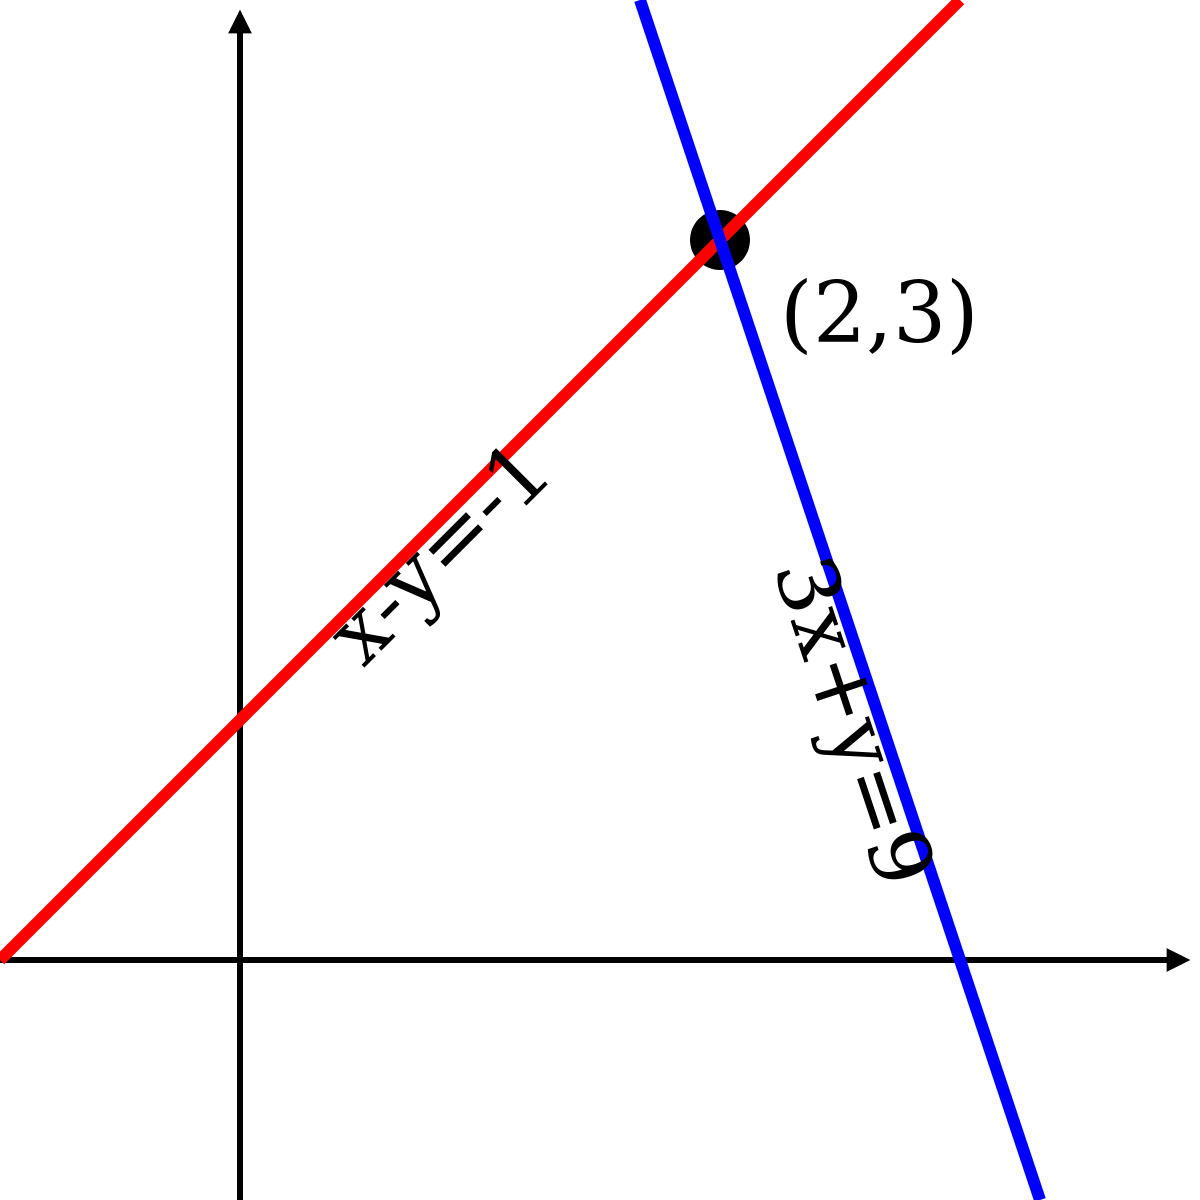
\includegraphics[width=4cm]{Images/1200px-Intersecting_Lines.svg.png}
    \caption{à 2 inconnues}
    \label{fig:Graphe 2 inconnues}
\end{figure}
\begin{definition}
    Un système linéaire est une collection de une ou plusieurs équations linéaires
    \begin{equation}
        \begin{cases}
            a_{1,1}x_1 + ... + a_{1,n}x_n = b_1\\
            a_{m,1}x_1 + ... + a_{m,n}x_n = b_m
        \end{cases}
    \end{equation}
\end{definition}
\begin{theorem}
    Un système linéaire a zéro, une ou une infinité de solutions
\end{theorem}
\begin{theorem}[Opérations élémentaires]
    Ces opérations ne changent pas les solutions du système :
    \begin{itemize}
        \item Permuter 2 équations
        \item Multiplier une équation par un nombre non nul
        \item Soustraire un multiple d'une équation à une autre
    \end{itemize}
\end{theorem}
\begin{definition}
    Pour une matrice de taille m \(\times\) n, on appelle \textcolor{red}{coefficient principal} d'une ligne non-nulle le coefficient non-nul le plus à gauche dans la ligne
\end{definition}
Une matrice est sous forme \underline{échelonnée} si
\begin{enumerate}
    \item Toutes les lignes non-nulles (s'il y en a) sont en bas
    \item Le coefficient principal de toute ligne se trouve à droite du coefficient principal de la ligne au dessus, \underline{et}
    \item Tous les coefficients d'une colonne sous un coefficient principal sont nuls
    \[ \begin{pmatrix}
            \textcolor{red}{a_{1,1}} & a_{1,2} & a_{1,3} & b_1 \\ 
            0 & \textcolor{red}{a_{2,2}} & a_{2,3} & b_2\\
            0 & 0 & 0 & 0
        \end{pmatrix} \]
\end{enumerate}
Une matrice qui satisfait \underline{en plus} les deux conditions ci-dessous est sous forme \underline{échelonnée réduite} :
\begin{enumerate}
    \item Le coefficient principal de chaque ligne vaut 1 \underline{et}
    \item Les coefficients principaux sont les seuls éléments non-nuls de leur colonne
    \[ \begin{pmatrix}
            \textcolor{red}{1} & 0 & a_{1,3} & b_1 \\ 
            0 & \textcolor{red}{1} & a_{2,3} & b_2\\
            0 & 0 & 0 & 0
        \end{pmatrix} \]
\end{enumerate}
\begin{definition}
    Deux matrices sont \underline{équivalentes par les lignes} si on peut obtenir l'une à partir de l'autre via une séquence d'opérations élémentaires sur les lignes
\end{definition}
\begin{remark}
    Toute matrice non-nulle est équivalente par les lignes avec plusieurs  matrices échelonnées
\end{remark}
\begin{theorem}
    Toute matrice échelonnée est équivalente par les lignes à \underline{exactement une} matrice échelonnée réduite
\end{theorem}
\begin{strat}
    Résoudre un système d'équations
    \begin{enumerate}
        \item Ecrire la matrice augmentée du système
        \[ \begin{pmatrix}
            a_{1,1} & a_{1,2} & a_{1,3} & b_1 \\ 
            a_{2,1} & a_{2,2} & a_{2,3} & b_2\\
            a_{3,1} & a_{3,2} & a_{3,3} & b_3
        \end{pmatrix} \]
        \item Mettre la matrice sous forme échelonnée à l'aide des opérations élémentaires
        \[ \begin{pmatrix}
            a_{1,1} & a_{1,2} & a_{1,3} & b_1 \\ 
            0 & a_{2,2} & a_{2,3} & b_2\\
            0 & 0 & a_{3,3} & b_3
        \end{pmatrix} \]
        \begin{itemize}
            \item Si \( a_{3,3} = 0\) et \(b_3 = 0 \), alors le système aura une infinité de solution avec une variable libre
            \item Si \( a_{3,3} = 0\) et \(b_3 \neq 0 \), alors le système n'aura aucune solution
        \end{itemize}
        \item Continuer de façon à obtenir une matrice échelonnée réduite
        \[ \begin{pmatrix}
            1 & 0 & 0 & b_1 \\ 
            0 & 1 & 0 & b_2\\
            0 & 0 & 1 & b_3
        \end{pmatrix} \]
        \item Réécrire le système d'équation
        \item Exprimer chaque variable liée en fonction des variables libres
    \end{enumerate}
\end{strat}
\section{Equations vectorielles}
\subsection{Propriétés algébriques de \( \mathbf{R}^n \) }
\begin{multicols}{2}
    \begin{itemize}
        \item \( \overrightarrow{u} + \overrightarrow{v} =  \overrightarrow{v} + \overrightarrow{u} \)
        \item \( \overrightarrow{u} + \overrightarrow{0} = \overrightarrow{u}\)
        \item \(\overrightarrow{u} + \overrightarrow{-u} = \overrightarrow{0}\)
    \end{itemize}
\columnbreak
\begin{itemize}
    \item \( a(\overrightarrow{u} + \overrightarrow{v}) = a\overrightarrow{u}  + a\overrightarrow{v} \)
    \item \( (a + b)\overrightarrow{u} = a\overrightarrow{u} + b\overrightarrow{u} \)
    \item \(a(b\overrightarrow{u}) = (ab)\overrightarrow{u}\)
\end{itemize}
\end{multicols}
\subsection{Combinaison linéaire}
\( \overrightarrow{y} = c_1\overrightarrow{v}_1 + c_2\overrightarrow{v}_2 ... + c_p\overrightarrow{v}_p \) 
\begin{definition}
    \(Vect(\overrightarrow{v}_1, ..., \overrightarrow{v}_p)\) est le sous ensemble de \(R^n\) engendré par les vecteurs
\end{definition}
\begin{figure}[htp]
    \centering
    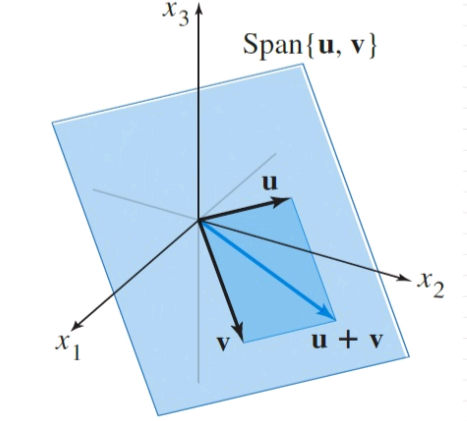
\includegraphics[width=4cm]{Images/Span.png}
    \caption{Vect()}
    \label{fig:span}
\end{figure}
On peut résoudre : \( A\overrightarrow{x} = \overrightarrow{b}\) pour trouver les composantes \(C_x\) (solution particulière) ou \( A\overrightarrow{x} = \overrightarrow{b}\) pour trouver la solution homogène \newpage
Cela donnera une solution de la forme : \(\begin{pmatrix}
    x \\
    y \\
    0
\end{pmatrix} + t\begin{pmatrix}
    a \\
    b \\
    1
\end{pmatrix} \)  pour \(x_3\) libre \\
\begin{figure}[htp]
    \centering
    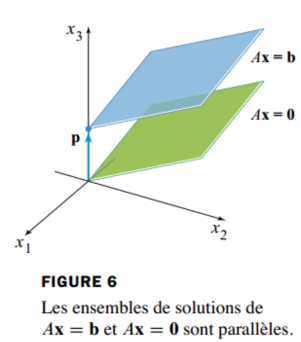
\includegraphics[width=5cm]{Images/Paralleles.png}
    \label{fig:parallele}
\end{figure}
\subsection{Indépendance linéaire}
On dit qu'une famille de vecteurs est linéairement indépendante si :
\[ x_1v_1 + x_2v_2 + ... + x_nv_n = 0\]
admet la solution triviale comme unique solution (ou liés si les \(x_n\) ne sont pas tous nuls en même temps)\\
On peut résoudre le système homogène \( A\overrightarrow{x} = \overrightarrow{0}\) pour savoir si nos vecteurs sont linérairement dépendants : \\
Si la seule solution possible est la solution triviale (0) alors les vecteurs engendrent \(R^x\) (si nous avons suffisament de vecteurs) et on peut créer n'importe quel vecteur dans la dimension x
\begin{figure}[htp]
    \centering
    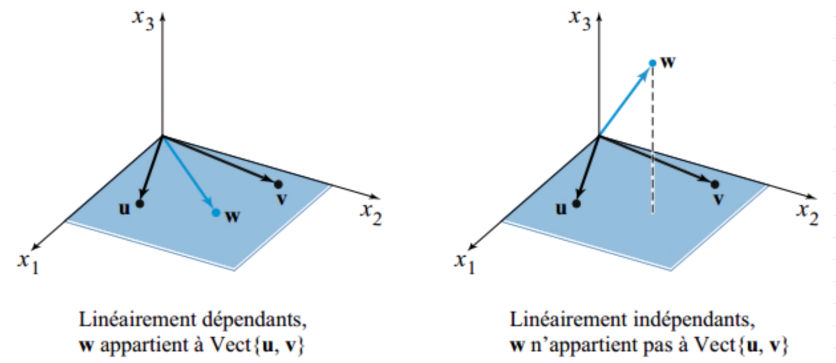
\includegraphics[width=12cm]{Images/linéarité.png}
    \label{fig:linearite}
\end{figure}
\begin{remark}
    Si on a p vecteurs dans une dimension \(R^n\) avec p \(>\) n, alors la famille de vecteurs est forcément linéairement dépendante 
\end{remark}
\section{Applications linéaires}
On peut voir A\(\overrightarrow{x}\) = T(x) comme une fonction/application qui va de \(R^n\) à \(R^m\), avec n le nombre de colonnes de A et m le nombre de lignes
\begin{definition}
    Une application est linéaire si :
    \begin{itemize}
        \item \(T(\overrightarrow{u} + \overrightarrow{v}) = T(\overrightarrow{u}) + T(\overrightarrow{v})\) \\
        \underline{et}
        \item \(T(c\overrightarrow{u}) = cT(\overrightarrow{u}) \)
    \end{itemize}
    Toutes les applications matricielles sont linéaires
\end{definition}
\begin{theorem}
    Soit T une application linéaire, il existe une unique matrice A telle que T(x) = A\(\overrightarrow{x}\)
    De plus, A sera donné par : 
    \[ A = [ T(\overrightarrow{e}_1) + T(\overrightarrow{e}_2) + ... + T(\overrightarrow{e}_n)] \]
    Avec \( \overrightarrow{e}_1, \overrightarrow{e}_2,\ ..., \overrightarrow{e}_n \) les colonnes de la matrice identité
\end{theorem}
\subsection{Injectivité et Surjectivité}
\begin{definition}
    Une matrice est \underline{injective} si ses colonnes sont indépendantes 
\end{definition}
\begin{definition}
    Une matrice est \underline{surjective} si elle engendre $\mathbf{R}^n$ 
\end{definition}
\subsection{Produit matriciel}
\begin{definition}
    Soit deux matrices \[ A \in \mathbf{R}^{m\times{n}},  B \in \mathbf{R}^{n\times{p}} \]
    Le produit AB compatible est défini comme : (utile pour prouver les autres propriétés !)
    \[ AB_{ij} = \sum^{n}_{k=1} A_{ik} \cdot B_{kj} \]

    AKA ligne de A $\times$ colonne de B
\end{definition}
\begin{theorem}
Propriétés du produit matriciel :
\begin{multicols}{2}
\begin{itemize}
    \item A(BC) = (AB)C
    \item A(B + C) = AB + AC
    \item (B + C)A = BA + CA
    \columnbreak
    \item r(AB) = (rA)B = A(rB)
    \item $I_m$A = A = A$I_n$
    \item \textcolor{red}{En général} AB $\neq$ BA
\end{itemize}
\end{multicols}
\end{theorem}
\subsection{Matrice transposée}
Soit A $ \in \mathbf{R}^{n \times m}$, alors $A^T \in \mathbf{R}^{m \times n}$ telle que $(A^T)_{ji} = A_{ij}$ \\\\
Propriétés :
\begin{itemize}
    \item $(A^T)^T = A$
    \item $(A + B)^T = A^T + B^T$
    \item $(rA)^T = rA^T$
    \item $(AB)^T = B^TA^T \implies (A_1A_2...A_k)^T = A_k^T...A_2^TA_1^T$ 
\end{itemize}
\subsection{Inverse d'une matrice}
Pour qu'une matrice soit inversible il faut (Soit A n $\times$ n):
\begin{itemize}
    \item A carrée
    \item det(A) $\neq$ 0 / rg(A) = 3
    \item A engendre $R^n$ \underline{et} Colonnes indépendantes
\end{itemize}
\begin{definition} Définition de la matrice inverse :
    \[ AA^{-1} = A^{-1}A = I_n\]
\end{definition}
\begin{remark}
    Trouver l'inverse d'une matrice revient à échelonner la matrice augmentée $ \begin{pmatrix}
        A & I_n
    \end{pmatrix} $. En fait, on cherche la série d'opérations élémentaires qui vont transformer $ A $ en $ I_n $. On retient donc ces opérations à droite (sur notre $ I_n $,) jusqu'à ce que $ A $ soit égale à la matrice identitée à gauche. On obtient $ \begin{pmatrix}
        I_n & A^{-1}
    \end{pmatrix} $ \\
    Cela revient à résoudre l'équation : \[ AA^{-1} = I_n \] avec les composantes de $A^{-1}$ inconnues, et donc Ax = $I_n$ qu'on résoud en echelonnant comme habituellement \\\\
    Pour A $\in \mathbf{R}^{2 \times 2} \begin{pmatrix}
        a & b \\
        c & d
    \end{pmatrix}$ :
    \[ A^{-1} = \frac{1}{det(A)} \begin{pmatrix}
        d & -b \\
        -c & a
    \end{pmatrix}\]
    Avec det(A) = ad - bc
\end{remark}
\begin{theorem}
    Pour tout b $\in \mathbf{R}^n$, $A\overrightarrow{x} = \overrightarrow{b}$ a une unique solution x = $A^{-1}b$ si A est inversible
\end{theorem}
Propriétés :
\begin{itemize}
    \item $(A^{-1})^{-1} = A$
    \item $(AB)^{-1} = B^{-1}A^{-1} $
    \item $ (A^T)^{-1} = (A^{-1})^T \implies (A_1A_2...A_k)^{-1} = A_k^{-1}...A_2^{-1}A_1^{-1} $
\end{itemize}

\subsection{Déterminants}

\begin{theorem}
    Propriétés :
    \begin{itemize}
        \item $ det(AB) = det(A) \cdot det(B) $
        \item $ det(A) = det(A^T) $
        \item Soit $ C $ une matrice triangulaire. $ det(C) = \prod a_{ij}, i = j $ (multiplier les coeffs de la diagonale)
        \item $det(A^x) = (det(A))^x \implies det(A^{-1}) = \frac{1}{det(A)}$
        \end{itemize}
\end{theorem}

\begin{theorem}
Soit A une matrice carrée. On applique l'opération O à A pour obtenir B.
    \begin{itemize}
        \item O = permuter deux lignes $ \implies det(B) = -det(A) $
        \item O = ajouter un multiple d'une ligne à une autre $ \implies det(B) = det(A) $
        \item O = multiplier une ligne par un coef $ k $ $ \implies det(B) = kdet(A) $
    \end{itemize}
\end{theorem}

\begin{theorem}
$ \newline \newline $
\textbf{A inversible} $ \Leftrightarrow $
\begin{itemize}
    \item les colonnes de $ A $ sont indépendantes.
    \item l'application linéaire $ \textbf{x} \rightarrow \textbf{Ax} $ est bijective.
    \item $ A^T $ est inversible.
    \item ...
\end{itemize}
\end{theorem}
\begin{remark}
    Pour calculer le déterminant d'une matrice, on peut d'abord l'échelonner puis multiplier le déterminant de sa forme échelonnée par les déterminants de chaque matrice élémentaire utilisée lors de l'échelonnement (complexité de $ n^3 $ au lieu de $ n! $).
\end{remark}

\begin{theorem}
$ \newline $
A matrice $ 2\times 2 \implies $ aire du parallélogramme défini par colonnes de A $ = \lvert det(A) \lvert $ \\
A matrice $ 3\times3 \implies $ volume du parallélogramme défini par colonnes de A $ = \lvert det(A) \lvert $
\end{theorem}

\subsection{Espaces vectoriels}

\begin{definition}
    Un espace vectoriel est un ensemble homogène non vide composé d'objets appelés vecteurs de l'espace (matrices, scalaires, polynômes, peu importe). On définit deux opérations : l'addition et la multiplication par un scalaire.
\end{definition}

\begin{definition}
    Un sous-espace vectoriel H est un sous-ensemble d'un espace V qui vérifie les propriétés suivantes.
\end{definition}

\begin{itemize}
    \item Le vecteur nul de V appartient à H.
    \item $ \mathbf{u} $ and $ \mathbf{v} \in H \implies \mathbf{u} + \mathbf{v} \in H $
    \item $ \mathbf{u} \in H \implies c\cdot \mathbf{u} \in H $
\end{itemize}

\subsection{Kernel et Image}

\begin{definition}
    Le noyau (ou kernel) d'une matrice A est l'ensemble des vecteurs qui sont une solution de $ A\mathbf{x} = \mathbf{0} $.
\end{definition}

\begin{definition}
    L'image d'une matrice A est l'ensemble des vecteurs qui sont une solution de $ A\mathbf{x} = \mathbf{b} $.
\end{definition} 
Application linéaire : \\
Ker(A) = $\begin{Bmatrix}
    0
\end{Bmatrix}$
si l'application A est injective \\
Im(A) = $R^n$ si l'application A est surjective
\subsection{Bases}
Une famille de vecteurs de V est une base de H si la famille est libre et engendre H (vérifier le détérminant par exemple) \\\\
La base canonique de $R^n$ est la matrice identité
\begin{itemize}
    \item \textbf{Trouver une base de H} \\
Il faut enlever les vecteurs linéaires à d'autres vecteurs et ne garder que ceux qui sont linéairement indépendant (ou rajouter des vecteurs)
    \item \textbf{Trouver une base de Ker(A)} \\
    Echelonner la matrice et regarder les lignes $(x_1 = ...)$ et écrire les $x_n$ indépendants
    \item \textbf{Trouver une base de Im(A)} \\
    Echelonner la matrice et regarder les colonnes avec un pivot, prendre les vecteurs correspondants à ces colonnes dans la matrice de base
\end{itemize}
\subsection{Système de coordonnées}
Pour chaque base, il existe une unique combinaison de scalaire pour définir un vecteur
\[ \overrightarrow{x} = c_1b_1 + c_2b_2 + ... + c_nb_n \]
\begin{itemize}
    \item $[x]_{B} = \begin{bmatrix}
        c_1 \\
        ... \\
        c_n
    \end{bmatrix}$ = $(P_B)^{-1} \overrightarrow{x}$ \qquad avec $P_B = [b_1\ ...\ b_n]$
    \item $[x]_{Bcan} = \overrightarrow{x} = \begin{bmatrix}
        x_1\\
        ... \\
        x_n
    \end{bmatrix}$
\end{itemize}
\subsection{Isomorphisme}
Le pouvoir de transformer ce qui n'est pas vectoriel en un vecteur de $R^n$\\ (ex $P^3 -> R^4)$
\subsection{Rang}
\begin{itemize}
    \item Rang(A) = dim(Im(A))
    \item Rang(A) $\leq$ m \qquad (Im(A) est un sous espace de $R^m$)
    \item Rang(A) $\leq$ n \qquad (Im(A) est engendré par n vecteurs)
\end{itemize}
\begin{theorem}
    Théorème du rang : Rang(A) + dim(Ker(A)) = n \qquad (n est le nombre de colonnes)
\end{theorem}
\begin{theorem}
    Rang(A) = Rang($A^T$) \qquad (dim(Im(A)) = dim(Lgn(A)))
\end{theorem}
\begin{remark}
    Lemme : Si B est inversible, alors Im(A) = Im(AB)
\end{remark}
\begin{theorem}
    dimA$^T$ + dimKerA = n 
    dimImA + dimKerA$^T$ = m\\avec $R^{m x n}$
\end{theorem}
\subsection{Changement de base} 
$[x]_C = P_{C \leftarrow B}[x]_B $ avec $P_{C \leftarrow B} = [[b_1]_C [b_2]_C ... [b_n]_C] $ \\\\
$P_{B \leftarrow C} = P_{C \leftarrow B}^{-1}$ \\\\
Pour les fonctions :
\[ [T]_B = P_{B \leftarrow C}[T]_CP_{C \leftarrow B}\]
\subsection{Vecteur et Valeurs propres}
Valeur propre : $A\overrightarrow{u} = \lambda\overrightarrow{u} $ avec $\lambda$ la valeur propre \\\\
$ \implies (A - \lambda I_n) = 0$ pour trouver les valeurs propres ou $det(A - \lambda I_n) = 0$ \\\\
Vecteur propre : Echelonner $(A - \lambda I_n)$
\begin{theorem}
    Les vecteurs propres de valeurs propres différentes sont linéairement indépendants
\end{theorem}
\begin{theorem}
    Les valeurs ont des multiplicités :
    \begin{itemize}
        \item Algébrique : Le nombre de fois qu'elles sont racines
        \item Géométrique : Le nombre de vecteurs propres qu'elles engendrent / DimKerA
    \end{itemize}
    Multiplicité géométrique $\leq$ Multiplicité algébrique
\end{theorem}
\begin{remark}
    Trace(A) = somme des valeurs propres
\end{remark}
\begin{definition}[Matrices semblables]
    A et B sont semblables si B = $PAP^{-1}$\\
    Cela définit une relation d'équivalence et leurs polynômes caractéristiques sont égaux
\end{definition}
\subsection{Diagonalisation}
A est diagonalisable si A = $PDP^{-1}$ \\
D est la matrice diagonale contenant les valeurs propres, et P la matrice associée contenant les vecteurs propres
\begin{remark}
    A est diagonalisable si pour toutes les valeurs propres, Mult.Alg. = Mult.Geo.
\end{remark}
\section{Orthogonalité et méthode des moindres carrés}
\subsection{Produit scalaire}
$\overrightarrow{u}\cdot\overrightarrow{v} = u_1v_1 + u_2v_2 + ... + u_nv_n$\\\\
$\overrightarrow{u}\cdot\overrightarrow{v} = ||u||||v||cos\phi$
\subsection{Norme}
$||\overrightarrow{v}|| = \sqrt{v_1^2 + v_2^2 + ... + v_n^2}$
\subsection{Vecteur unitaire}
$\overrightarrow{u} = \frac{1}{||\overrightarrow{v}||}\overrightarrow{v}$
\subsection{Distance}
$Dist(u,v) = ||\overrightarrow{u} - \overrightarrow{v}||$
\subsection{Orthogonalité}
\begin{theorem}
    $\overrightarrow{u} \cdot \overrightarrow{v} = 0$
\end{theorem}
\begin{theorem}
    $||u + v||^2 = ||u^2|| + ||v^2||$
\end{theorem}
\subsection{Complément orthogonal}
$W^{\perp}$(SEV) c'est l'ensemble des vecteurs de $R^n$ qui sont orthogonaux à tous les vecteurs de W
\begin{theorem}
    $(W^{\perp})^{\perp}$ = W
\end{theorem}
\begin{itemize}
    \item $(Ker A)^{\perp} = ImA^T$
    \item $(ImA)^{\perp} = KerA^T$
    \item $(KerA^T)^{\perp} = ImA$
    \item $(ImA^T)^{\perp} = KerA  $
\end{itemize}
\subsubsection{Familles et bases orthognales}
Une famille est orthogonale si chaque vecteur y appartenant est orthogonal à tous les autres. \\\\
Si une base est une famille orthogonale alors la base est orthogonale
\newline \newline 
Pour tout y = $c_1u_1 + c_2u_2 + ... + c_nu_n$ \\
$c_i = \frac{y \cdot u_i}{u_i \cdot u_i}$

\subsection{Projection orthogonale}
$proj_W(y) = \hat{y} = \frac{y \cdot u_1}{u_1 \cdot u_1}u_1 +  \frac{y \cdot u_2}{u_2 \cdot u_2}u_2 + ...$\\\\
$proj_{W^{\perp}}(y) = y - proj_W(y)$\\\\
Si on a une base orthonormée alors : \\\\
$proj_W(y) = \hat{y} = (y \cdot u_1)u_1 + (y \cdot u_2)u_2 + ...$

\subsection{Base orthonormale}
Soit une matrice U avec des colonnes orthonormées alors
\begin{itemize}
    \item $U^TU = I$
    \item $||Ux|| = ||x||$
    \item $(Ux) \cdot (Uy) = x \cdot y$
\end{itemize}
$proj_W(y) = UU^Ty$
\subsubsection{Matrice orthogonale}
U est orthogonale si elle est carrée et ses colonnes sont othornormées
\begin{itemize}
    \item $U^{-1} = U^T$
    \item $U^TU = UU^T = I$
\end{itemize}
\subsection{Gram-Schmidt}
On a B = {$x_1, x_2, ...$} qu'on souhaite orthonormalisé
\begin{enumerate}
    \item On pose $u_1 = x_1\frac{1}{||x_1||}$ et W = {$u_1$}
    \item $v_2 = x_2 - proj_W(x_2) = x_2 - (x_2 \cdot u_1)u_1$
    \item $u_2 = x_2\frac{1}{||x_2||}$ et W = {$u_1, u_2$}
    \item ...
\end{enumerate}
\subsection{Moindres carrés}
On pose A = [$x_1$ $x_2$ ...], Q = [$u_1$ $u_2$ ...] et R = $\begin{pmatrix}
    ||x_1|| & u_1 \cdot x_2 & u_1 \cdot x_3 & ... \\
    0 & ||v_2|| & u_2 \cdot x_3n & ...\\
    0 & 0 & ||v_3|| & ... \\
    0 & 0 & 0 & ...
\end{pmatrix}$
On a $|det(a)|$ = Volume du parallélépipède engendré \\\\
On cherche Ax aussi proche que possible de b = $\hat{b}$ = A$\hat{x}$ $\rightarrow$ 2 méthodes
\subsubsection{Equations normales}
$A^TA\hat{x} = A^Tb$
\subsubsection{Factorisation QR}
$R\hat{x} = Q^Tb$
\subsection{Regréssion linéaire (Droite graphique)}
On cherche une droite tel que y = $\beta_1x + \beta_2$
On pose :
A =$ \begin{pmatrix}
    1 & x_1 \\
    1 & x_2 \\
    1 & ... \\
\end{pmatrix}$ 
$\beta $$= \begin{pmatrix}
    \beta_2 \\
    \beta_1
\end{pmatrix} $ 
et y = $\begin{pmatrix}
    y_1 \\
    y_2 \\
    ...
\end{pmatrix}$ \\\\
et $A^TA\beta$ = $A^Ty$

\subsection{Décomposition SVD}

Soit A une matrice de dimension $ m \times n $.\\\\
On cherche :
\begin{itemize}
    \item une matrice \textbf{orthonormée} U de dimension $ m \times m $.
    \item une matrice \textbf{diagonale} V de dimension de $ A $.
    \item une matrice \textbf{orthonormée} V de dimension $ n \times n $.
\end{itemize}

\subsubsection{Recherche des valeurs et vecteurs propres}

Pour commencer, il nous faut chercher les vecteurs propres \textbf{normalisés} de $ A \cdot A^T $ ou de $ A^T \cdot A $. Comment choisir entre les deux ?\\\\
Jusqu'ici je pense que le mieux est de choisir le produit qui donne la matrice la plus petite (on préfèrera chercher les vecteurs propres d'une matrice $ 2\times2 $ puis trouver un vecteur orthogonal aux deux autres que de chercher les vecteurs propres d'une matrice $ 3\times 3$).\\
Si nous avons calculer $ A \cdot A^T $, nous avons les colonnes de U.
Si nous avons calculer $ A^T \cdot A $, nous avons les colonnes de V.

\subsubsection{Calculer la matrice $ \sigma $}

La matrice $ \sigma $ est une matrice dont les entrées diagonales sont les seules non-nulles et égales à la racine carrée des valeurs propres précédemment trouvées.

\subsubsection{Calculer la matrice manquante}

Ensuite, il nous faut trouver un vecteur de V ou de U en fonction du choix de 1) orthogonal aux deux autres.\\
Parfois on trouve directement un vecteur en regardant les deux autres, sinon il faut utiliser Gram Schmidt.

\end{document}
